The mathematical software systems to be integrated via the MitM approach have so far been computation-oriented, e.g., computer algebra systems.
Their API theories typically declare types and functions on these types (the latter including constants seen as nullary functions).
Even though database systems differ drastically from these in many respects, they are very similar at the MitM level: a mathematical database defines
\begin{compactitem}
 \item some types: each table's schema is essentially one type definition,
 \item many constants: each table entry is one constant of the corresponding type.
\end{compactitem}
Thus, we can reuse many of the same concepts.
In particular, the API theories must contain definitions of the database schemas. 

Apart from standard software engineering tasks, this leaves three conceptual problems we had to solve:
\begin{compactenum}[\bf P1]
\item Turn the database schemas and tables into \ommt theories and declarations. 
\item Lift data in \emph{physical} representation (as records of the
  underlying database) to \ommt object in \emph{semantic} representation.
\item Translate semantic queries to queries about physical representations so
  that they can be executed directly on the database without loading the entire theory into
  \mmt.
\end{compactenum}
We deal with \textbf{P1} in Section~\ref{sec:vt}, with \textbf{P2} in Section~\ref{sec:vt:codec}, and with \textbf{P3} in Section~\ref{sec:qmt}. 

In this \papertype, we focus on \lmfdb as an example, of which we give an overview in Section~\ref{sec:lmfdb}.
However, our methods are general enough to apply to many other mathematical databases such as OEIS, or findstat.

 \subsection{LMFDB Overview}\label{sec:lmfdb}

 The ``L-Functions and Modular Forms Database'' (\lmfdb~\cite{lmfdb}) is a large database, storing among other mathematical objects millions of L-Functions, modular forms and curves, along with their properties.
Technically, it uses a MongoDB database with a Python web frontend.

\lmfdb has several sub-databases, e.g., for elliptic curves or transitive groups. 
Within each of these, every object is stored as a single JSON record.
Figure~\ref{fig:lmfdbexample} shows an example: each property of this JSON object corresponds to a property of the underlying mathematical object. 
For example, the \identifier{degree} property --- here $1$ --- of the JSON objects corresponds to the degree of modular parametrization of the underlying elliptic curve. 

\begin{figure}[ht]\centering
\begin{lstlisting}[language=json]
{
    "degree": 1,
    "x-coordinates_of_integral_points": "[5,16]",
    "isogeny_matrix": [[1,5,25],[5,1,5],[25,5,1]],
    "label": "11a1",
    "_id": "ObjectId('4f71d4304d47869291435e6e')",
    ...
}
\end{lstlisting}
  \caption[An elliptic curve from \lmfdb]{
    Part of an elliptic curve in \lmfdb (some fields omitted for brevity)
  }
  \label{fig:lmfdbexample}
\end{figure}

Other properties are more complex: the value of the \identifier{isogeny\_matrix} property is a list of lists representing a matrix. 
This disconnect between JSON encoding and mathematical meaning can become much more severe, e.g., the \identifier{x-coordinates\_of\_integral\_points} field is semantically a list of integers but (due to the sizes limits on integers) is encoded as a string.

The \lmfdb API \cite{lmfdbapi} exposes a querying interface that can be used either by humans via the web or programmatically via JSON-based GET requests over HTTP.
%\ednote{FR: I commented out a screenshot here because it doesn't seem to add much at this point of the paper.}
%A screenshot of the former interface can be seen in Figure~\ref{fig:apiscreenshot}. 
%
%\begin{figure}[ht]\centering
%  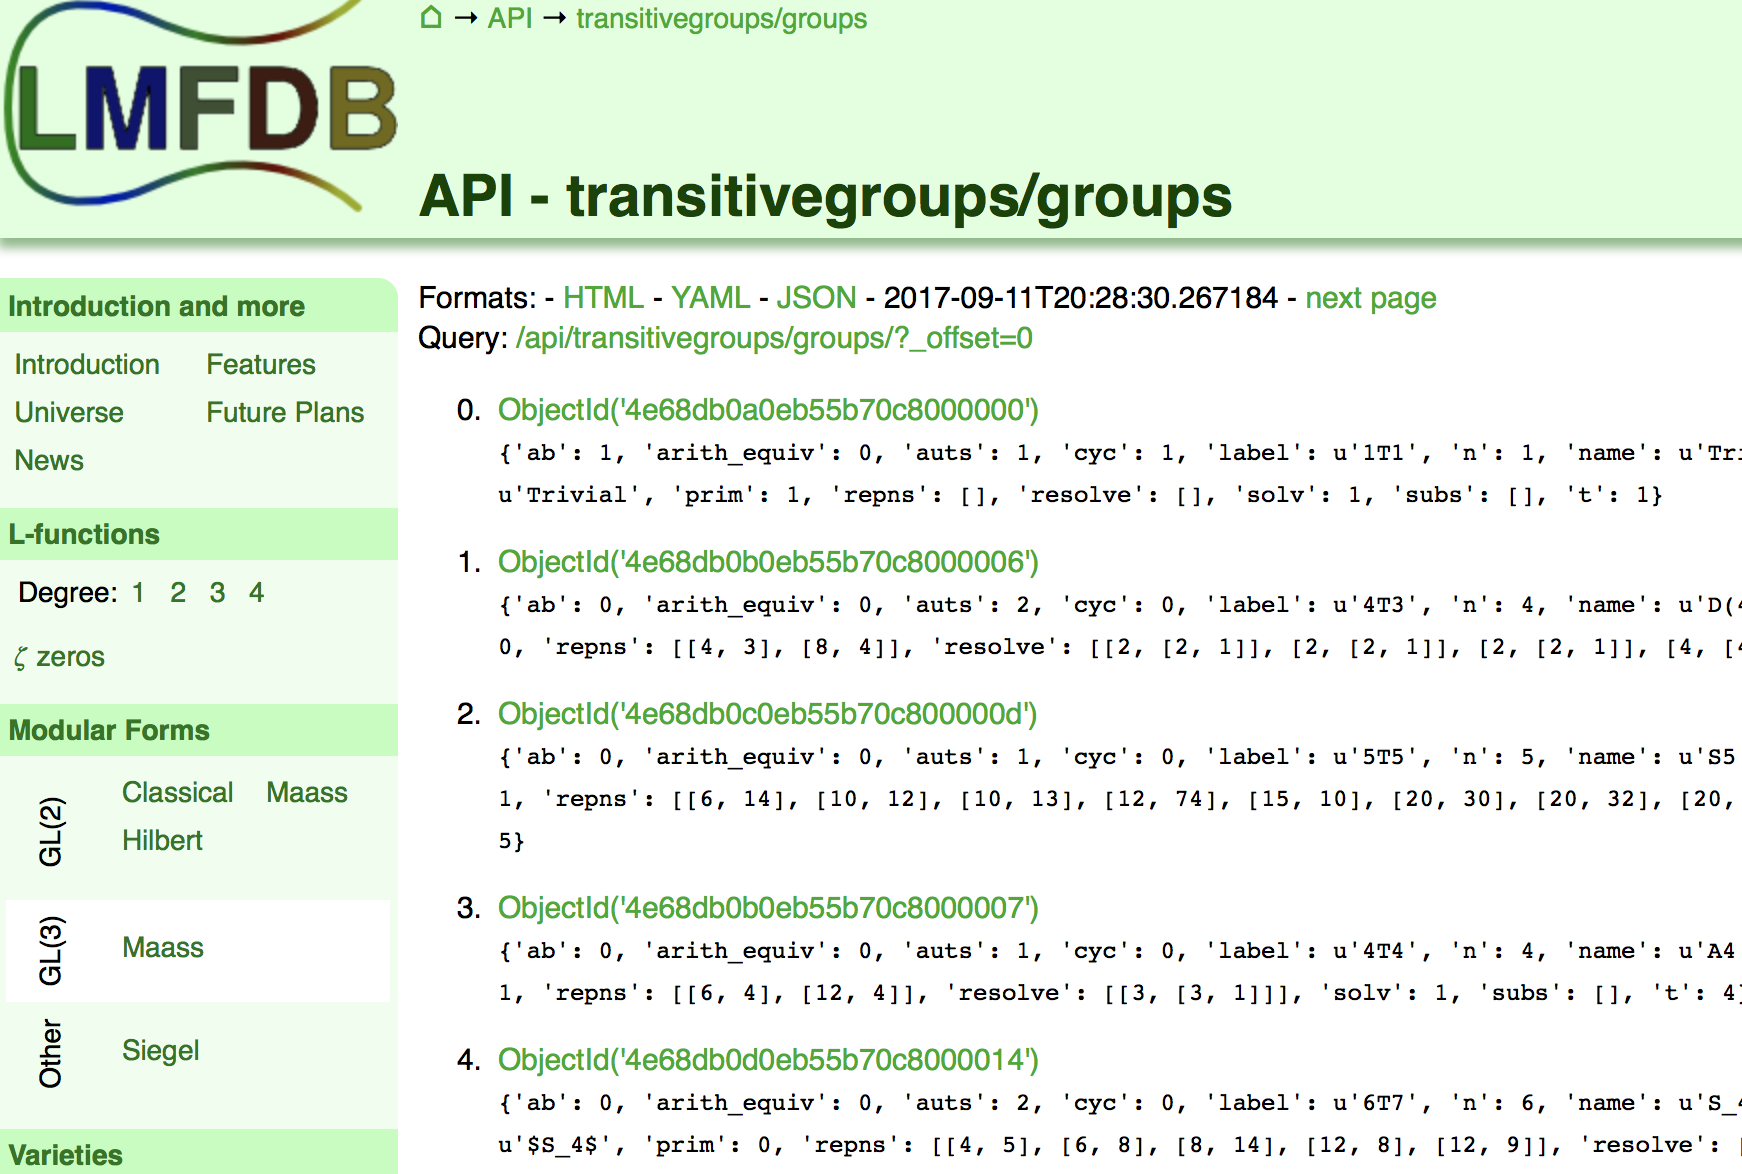
\includegraphics[width=0.97\textwidth,viewport=0 240 800 600 ,clip=true]{../MACIS17-vt/APIScreenshot}
%  \caption{The Web-Interface for the \lmfdb API.}\label {fig:apiscreenshot}
%\end{figure}
Queries must name the sub-database to be queried and consist of a set of key-value pairs that correspond to an SQL \texttt{where} clause.
However, while \lmfdb offers a programmable API for accessing its contents, this API sits at the level of the underlying MongoDB, and not the level of mathematical objects. 
For example, to retrieve all Abelian objects in the subdatabase of transitive groups, we expect to use the key-value pair \identifier{commutative}$ = $ \identifier{true}. 
However, these values need to be encoded to be understood by MongoDB.
We need to realize that the database schema actually uses the key \identifier{ab} for commutativity, that it has boolean values, and that the schema encodes \inlinecode{true} as \inlinecode{1}. 
Thus, the actual query to send is \url{http://www.lmfdb.org/api/transitivegroups/groups/?ab=1}. 

In this example, all steps are relatively straightforward. 
But in general, e.g. when searching for all elliptic curves with a specific isogeny matrix, this not only requires good familiarity with the mathematical background but also with the system internals of the particular \lmfdb sub-database; a skill set commonly found in neither research programmers nor average mathematicians.   

 \subsection[Virtual Theories]{\lmfdb as a Set of Virtual Theories}\label{sec:vt}

 The set of constants in a database table -- while finite -- can be arbitrarily large.
In particular, all \lmfdb tables%
\footnote{Technically, until July 2018, \lmfdb was implemented using MongoDB and comprises a set of sets (each one called a database) of JSON objects.
MongoDB allows each JSON object in a collection to be different (with a different schema), though in practice almost all objects in each collection had the same schema apart from some missing data components.
The schema for each collection had to be documented elsewhere, in an inventory, which since 2017 has been itself stored as a database within the LMFDB.
During 2018, however, work has been ongoing to migrate the LMFDB to use PostgreSQL (with a fixed schema for each table) as the underlying database, without any change to the external API.
In both cases, due to the conventions used, we can understand the LMFDB conceptually as a set of tables of a relational database, keeping in mind that every row is a tuple of arbitrary JSON objects.}
are just finite subsets of infinite sets, whose size is not limited by mathematical specifications but by computational power: the database holds all objects that users have computed so far and grows constantly as more objects are computed.
\lmfdb tables usually include a naming system that defines unique identifiers (which are used as the database keys) for these objects, and these identifiers are predetermined even for those objects that have not been computed yet.

Thus, it is not practical to fix a set of concrete API theories.
Instead, the API theories must be split into two parts: for each database table, we need
\begin{compactitem}
  \item a concrete theory called the \textbf{schema theory} that defines the schema  and other relevant information about the type of objects in the table and
  \item a virtual theory called the \textbf{database theory} that contains one definition for each value of that type (using the \lmfdb identifier as the name of the defined constant). 
\end{compactitem}

\begin{figure}[ht]\centering
    \begingroup
    \pgfdeclarelayer{background}
    \pgfdeclarelayer{foreground}
    \pgfsetlayers{background,foreground}
    
    \resizebox{\textwidth}{0.75\textwidth}{
      \begin{tikzpicture}[xscale=4,yscale=2.2]\footnotesize
        \begin{pgfonlayer}{foreground}
          \tikzstyle{human}    = [red,dashed,thick]
          \tikzstyle{withshadow}  = [draw,drop shadow={opacity=.5},fill=white]
          \tikzstyle{interface}   = [fill=blue!30]
          \tikzstyle{database}    = [cylinder,cylinder uses custom fill,
            cylinder body fill=yellow!50,cylinder end fill=yellow!50,
            shape border rotate=90,
            aspect=0.25,draw]
          
          % Ontology layer
          \node[thy] (numbers) at (0,1) {
            \begin{tabular}{lll}
              \multicolumn{3}{l}{\textsf{Numbers}}\\\hline\hline
              $\mathbb{Z}^{+}$        & : & \typett\\
              $\mathbb{Z}$            & : & \typett\\\hline
              \multicolumn{3}{l}{$\mathbb{Z}^{+} \subset \mathbb{Z}$}
            \end{tabular}
          };

          \node[thy] (matrices) at (1.5,1) {
            \begin{tabular}{lll}
              \multicolumn{3}{l}{\textsf{Matrices}}\\\hline\hline
              \plaintt{matrix} & : & $\typett \rightarrow \mathbb{Z}^{+}\rightarrow \mathbb{Z}^{+} \rightarrow \typett$
            \end{tabular}
          };

          \node[thy] (codecs) at (0.75,0) {
            \begin{tabular}{lll}
              \multicolumn{3}{l}{\textsf{Codecs}}\\\hline\hline
              \codectt                  & : & $\typett \rightarrow \typett$\\\hline
              \plaintt{standardInt}     & : & $\codectt\; \mathbb{Z}$\\
              \plaintt{standardMatrix}  & : & $\left\{T, n, m\right\} \codectt\; T \rightarrow \codectt\; \plaintt{matrix}(n, m, T)$\\
            \end{tabular}
          };

          \draw[include] (numbers) -- (matrices);
          \draw[include] (matrices) -- (codecs);
          
          \begin{pgfonlayer}{background}
            \node[draw=none,fill=green!30,rounded corners=1cm,fit=(numbers) (matrices) (codecs),inner sep=10pt] {};
          \end{pgfonlayer}
        
          % Model Layer
          \node[thy,fill=purple!30] (ec) at (2.25,-1.20) {
            \begin{tabular}{lll}
              \multicolumn{3}{l}{\textsf{Elliptic Curve}}\\\hline\hline
              \plaintt{ec}            & : & \typett\\\hline
              \plaintt{from\_record}  & : & $\plaintt{record} \rightarrow \plaintt{ec}$ \\\hline
              \plaintt{curveDegree}   & : & $\plaintt{ec} \rightarrow \mathbb{Z}$ \\
              \plaintt{isogenyMatrix} & : & $\plaintt{ec} \rightarrow \plaintt{matrix}(3, 3, \mathbb{Z})$ 
            \end{tabular}
          };

          \node[thy,interface] (ecschema) at (2.0,-2.5) {
            \begin{tabular}{lll}
              \multicolumn{3}{l}{\textsf{Elliptic Curve Schema Theory}}\\\hline\hline
              $\plaintt{degree}$            & \uri{?implements}  & \plaintt{curveDegree} \\
                                            & \uri{?codec}       & \plaintt{StandardInt} \\\hline
              $\plaintt{isogeny\_matrix}$   & \uri{?implements}  & \plaintt{isogenyMatrix} \\
                                            & \uri{?codec}       & $\plaintt{StandardMatrix}(3, 3, \plaintt{StandardInt})$ 
            \end{tabular}
          };

          % Database Layer
          \node[database] (mongodb) at (-.5,-2.5) {
            \textsf{\lmfdb Elliptic Curves}
          };

          \node[thy,interface] (dbtheory) at (0,-1.20) {
            \begin{tabular}{lllll}
              \multicolumn{5}{l}{\textsf{Elliptic Curve Database Theory}}\\\hline\hline
              \plaintt{11a1} & : & $\plaintt{ec}$ & $=$ & \dots\\
              \plaintt{11a2} & : & $\plaintt{ec}$ & $=$ & \dots\\
              \dots
            \end{tabular}
          };
          \draw[include] (matrices) to[bend left=20] (ec);
          \draw[include] (ec) -- (dbtheory);
          
          \draw[human,->] (dbtheory) -- node[right]{\scriptsize {lazily loads from}} (mongodb);
          \draw[human,->] (ecschema) -- node[right]{\scriptsize {implements}} (ec);
          \draw[human,->] (ecschema) -- node[above]{\scriptsize {describes}} (mongodb);
        \end{pgfonlayer}
      \end{tikzpicture}
    }
    \endgroup
  \caption[Virtual Theory Architecture]{
    Virtual theory for \lmfdb elliptic curves (some declarations omitted) 
  }
  \label{fig:vtarch}
\end{figure}
Conceptually, it is straightforward how to implement each \lmfdb table as a virtual MMT theory $V$: we use an initially empty concrete theory $C$, and whenever an identifier \textsf{id} of $V$ is requested, \mmt dynamically adds the corresponding declaration of \textsf{id} to $C$.
Because \mmt already abstracts from the physical realizations of persistent storage, we only have to implement a new storage instance that connects to \lmfdb, retrieves the JSON object with identifier \textsf{id}, and turns it into an \ommt declaration.

A sketch of our overall solution is given in Figure~\ref{fig:vtarch}.
The relevant parts of the MitM ontology comprise simple ones like numbers and matrices (in green) and \lmfdb-specific ones like elliptic curves (in red).
The remaining theories (in blue) form the \lmfdb API theories: the schema theory and the database theory, which we describe below.

\lmfdb's original technical realization, using MongoDB, did not require formalizing the schema of each table.
Instead, the tables were generated systematically and therefore followed an implicit schema that could --- in principle --- be obtained from the documentation or reverse-engineered from the tables.
Until 2017 the documentation of these implicit schemas was created and maintained manually by LMFDB developers, and as a result was incomplete and frequently out of date.
During 2017-2018 a new LMFDB Inventory was created, taking as its starting point both the manually prepared inventory (which contained human definitions and explanations of the content of each data field) and a new dynamically created schema obtained by analysis of the data in each collection.
This process, which was both necessitated by the requirements of the Math-in-the-Middle approach and made possible in practice through the provision of research software engineers funded by ODK, revealed numerous inconsistencies in the LMFDB data which developers have since been able to address.
Moreover, having this detailed schema for each collection in the MongoDB databases also fed in to the migration process, expected to be complete by August 2018, in which the MongoDB free-format collections are being replaced by PostgreSQL tables, each of which has a completely specified and formalized schema.

Note that (and here \lmfdb critically differs from, e.g., the OEIS), the mathematical definitions and concepts involved in the LMFDB data and tables are extremely deep so that reverse-engineering the associated schemas from the data itself is only possible in practice with the aid of experts.
As the first such table for which a formal schema was to be created, before the development of the new comprehensive Inventory, we chose one for which the existing documentation was most complete, and which originated with one of the current authors (John Cremona), who sat down with the Math-in-the-Middle team at an ODK workshop to formalize the corresponding schema in \ommt.
In the following, we will use this table as a running example.
Our methods extend immediately to any other table once its schema has been formalized.

Our formalization models elliptic curves in a very simple fashion by using an abstract type \identifier{ec}. 
The constructor \identifier{from\_record} takes an \mmt record and returns an elliptic curve. 
Properties of elliptic curves are formalized as functions out of this type.
We list only two here as examples: the \textsf{degree}, an integer, and the \textsf{isogeny\_matrix}, a $3 \times 3$ matrix of integers.
We omit the relevant axioms, which are not essential for our purposes here.
As usual for the MitM approach, the model of elliptic curves does not rely on \lmfdb, nor any other system, so that we can integrate other knowledge sources about elliptic curves or to future versions of the \lmfdb with changed structure. 


\subsection{Ascribing Encodings in Schema Theories}\label{sec:vt:codec}

If we ignore encoding issues, schema theories are straightforward: they contain one declaration of the same name for each field within an \lmfdb record. 
This specifies only the semantic type of each field and does not relate it to the MitM formalization.
To handle the encoding as a physical type, we annotate each declaration with the codec that the databases for the values of that field.
Moreover, to connect the schema theories to the MitM formalization, we additionally annotate each field with the corresponding property of elliptic curves from the MitM theory.
We can now understand the last unexplained parts of Fig.~\ref{fig:vtarch}.
\identifier{?implements} is the symbol used to annotate the metadatum, which MitM property a schema field corresponds to.
And \identifier{?codec} similarly annotates the codec to each field.

For example, the \identifier{degree} field implements the \identifier{curveDegree} property in the elliptic curve theory and uses the \identifier{StandardInt} codec.
Thus, the schema theories determine the entire relation between semantic and physical objects.

The database theory is a virtual theory and contains one declaration per \lmfdb record.
Given the URI of an object in the respective database, our \mmt backend for \lmfdb first retrieves the appropriate record from {\lmfdb} -- in the case of \identifier{11a1} this corresponds to retrieving the JSON found in Figure~\ref{fig:lmfdbexample}. 
Then, for each field, it uses the annotated codec (which is an \ommt expression) to build an actual codec (as a runnable Scala function) and runs its decoding function.
Next, it passes the resulting record to the \identifier{from\_record} constructor, which yields an elliptic curve in the MitM theories.
Finally, this elliptic curve is added as a new declaration in the database theory.

This example already shows that the virtual theories framework -- while conceptually slightly complex -- is declarative in the sense that it can be configured by supplying schema theories. 
This task only requires knowledge about the underlying mathematics (and how it is encoded in the MitM ontology; see Section~\ref{sec:knowls}), the encodings of the respective mathematical types in the basic data types of the underlying database, and  the data base schema.
In particular no knowledge of the \mmt internals or programming skills are needed and the prerequisite knowledge is exactly what \LMFDB contributors have (at the time they set up the particular sub-database). 

\subsection{Translating Queries}\label{sec:qmt}

 Recall that \mmt has a general-purpose Query Language called QMT~\cite{Rabe:qlfml12}, which allows users to find knowledge subject to even complex conditions. 
We continue by briefly addressing \textbf{P3}: query translation; for a complete discussion we refer the interested reader to \cite{twiesing:msc17}. 

In practice, most queries involving virtual theories so far have a shape similar to the one that \lmfdb supports: 
Finding all objects within a single sub-database for which a specific field has a specific value. 
As an example, consider again the query of finding all Abelian transitive groups. 
QMT has an \mmt-powered surface syntax, which can be used to express this query as:
\begin{lstlisting}[language=qmt,basicstyle=\small\sf]
x in (related to ( literal `lmfdb:db/transitivegroups?group ) by (object declares)) 
  | holds x (x commutative x *=* true)
\end{lstlisting}

The example consists of two parts, first we find all objects declared in the theory
interface theory \uri{lmfdb:db/transitivegroups?group} (line 1), and then we restrict this set of results to all those for which the \inlinecode{commutative} property is \inlinecode{true} (line 2). 
Notice that this the example shown here is the formal equivalent of the \lmfdb query shown in Section~\ref{sec:lmfdb}. 
The key difference is that this query does not require knowing the record structure of \lmfdb --
apart from knowing the proper sub-db, instead it only relies on knowing the mathematical
semantics (commutativity) of the query in question. 

Recall that to evaluate a query prior to the introduction of virtual theories, the \mmt system loaded the theory graph into main memory and then interleaved incremental flattening and query evaluation operations on the \mmt data structures until a result had been produced. 
But it is infeasible to first load all potentially relevant data into memory, and only then proceed with evaluation. 
This would require loading a copy of \lmfdb into main memory, something that virtual theories were designed to avoid. 

The low-level API of  \lmfdb and similar system provides a new approach for making queries towards virtual theories. 
First, the \mmt query is translated into a system-specific information-retrieval language --- in the case of \lmfdb\ this is currently a MongoDB-based syntax.
Next, this translated query is sent to the external API. 
Upon receiving the results, these are translated back into \ommt with the help of already existing functionality in the appropriate virtual theory backend.

This leaves just one problem unsolved --- translating queries into the system-specific API. 
Note that it is insufficient to simply translate queries as a whole: 
On the one hand a general QMT query may or may not involve a virtual theory, on the other hand, it may also involve several (unrelated) virtual theories. 
This makes it necessary to filter out queries involving virtual theories, and assign them to a specific backend, and then translate only these parts. 

Achieving this automatically is a non-trivial problem. 
Queries are inductive in nature, and one could attempt to intercept each of the intermediate results. 
However, this would require a check on each intermediate result to first determine if it comes from a virtual theory or not, and then potentially switching the entire evaluation strategy, leading to a computationally expensive implementation. 

Instead of intercepting each result, we extended the Query Language to allow users to annotate sub-queries for evaluation with a specific virtual theory backend. 
This allows the system to immediately know which parts of a query have to be evaluated in \mmt memory, and which have to be translated and sent to an external system. 
This turns the example above into:
\begin{lstlisting}[language=qmt]
use "lmfdb" for {*
  x in (related to ( literal `lmfdb:db/transitivegroups?group ) 
    by (object declares)) | holds x (x commutative x *=* true)
*}
\end{lstlisting}
Here, we have simply wrapped the entire query with a \inlinecode{use lmfdb} statement, indicating the query should be evaluated using \lmfdb. 

The encoding of this specific query can be achieved using codecs.
The query corresponds to the URL \url{http://www.lmfdb.org/api/transitivegroups/groups/?ab=1}. 
Next, the \lmfdb API returns a set of JSON objects corresponding to all Abelian transitive groups. 
These can then be decoded into \ommt objects using the procedure described in Section~\ref{sec:vt:codec}, i.e. for each field we look up the corresponding codec and use it to deconstruct the field, eventually creating an \mmt record. 
Afterwards, these \ommt terms can then be passed to the user as a result to the query. 

%%% Local Variables:
%%% mode: latex 
%%% mode: visual-line
%%% fill-column: 5000
%%% TeX-master: "report"
%%% End:



%  LocalWords:  sec:qmt Rabe:qlfml12 textbf twiesing:msc17 lmfdb mmt-powered lstlisting sec:knowls
%  LocalWords:  qmt,basicstyle ommt qmt
%  LocalWords:  compactitem oldpart realization formalizing lmfdb sec:vt ommt textbf ec emph 4,yscale 50,cylinder 0.25,draw 30,rounded 1cm,fit formalizations
%  LocalWords:  centering begingroup pgfdeclarelayer pgfsetlayers background,foreground
%  LocalWords:  resizebox textwidth textwidth tikzpicture xscale 4,yscale pgfonlayer
%  LocalWords:  tikzstyle red,dashed,thick withshadow draw,drop cylinder,cylinder hline
%  LocalWords:  50,cylinder 0.25,draw hline mathbb plaintt rightarrow rightarrow codectt
%  LocalWords:  rightarrow none,fill 30,rounded 1cm,fit thy,fill isogenyMatrix ecschema
%  LocalWords:  thy,interface isogeny mongodb dbtheory endgroup fig:vtarch sec:access
%  LocalWords:  sec:qmt colored colored colored colored formalized textit textsf textsf
%  LocalWords:  realizations formalization
%  LocalWords:  sec:sota lmfdb lmfdb lstlisting json ainvs iwp0 2adic_gens isogeny_matrix
%  LocalWords:  tamagawa_product 2adic_index anlist 4f71d4304d47869291435e6e vspace emph
%  LocalWords:  fig:lmfdbexample isogeny includegraphics textwidth fig:apiscreenshot
%  LocalWords:  centering summarize sec:mmtmitm ommt-encoded 4f71d4304d47869291435e6e
%  LocalWords:  serialization wrapfigure parametrization ednote textwidth,viewport texttt
%  LocalWords:  nullary compactitem compactenum ommt emph textbf textbf sec:qmt lmfdb qmt
%  LocalWords:  sec:lmfdb papertype
%  LocalWords:  sec:vt lmfdb ommt textit textit realized tikzpicture tabularx textwidth sec:access realizations emph wrapfigure vspace lstlisting lstinline
%  LocalWords:  hline hline rightarrow codectt mathbb multirow fig:codecs isogeny mathrm
%  LocalWords:  characterized noindent formalized fig:codecops plaintt plaintt begingroup
%  LocalWords:  pgfdeclarelayer pgfsetlayers background,foreground resizebox xscale ec
%  LocalWords:  4,yscale pgfonlayer tikzstyle red,dashed,thick withshadow draw,drop oding
%  LocalWords:  cylinder,cylinder 50,cylinder 0.25,draw none,fill 30,rounded 1cm,fit
%  LocalWords:  thy,interface ecschema draw,cloud,fit 4,withshadow,inner 4pt,purple
%  LocalWords:  mongodb dbtheory endgroup fig:vtarch colored colored colored colored
%  LocalWords:  fig:lmfdbexample textbf centering RabKoh:WSMSML13 sec:mmtmitm
%  LocalWords:  internalizes
